\documentclass{article}
\usepackage{fullpage}
\usepackage[utf8]{inputenc}
\usepackage{pict2e}
\usepackage{amsmath}
\usepackage{enumitem}
\usepackage{eurosym}
\usepackage{mathtools}
\usepackage{amssymb, amsfonts, latexsym, cancel}
\setlength{\parskip}{0.3cm}
\usepackage{graphicx}
\usepackage{fontenc}
\usepackage{slashbox}
\usepackage{setspace}
\usepackage{gensymb}
\usepackage{accents}
\usepackage{adjustbox}
\setstretch{1.35}
\usepackage{bold-extra}
\usepackage[document]{ragged2e}
\usepackage{subcaption}
\usepackage{tcolorbox}
\usepackage{xcolor, colortbl}
\usepackage{wrapfig}
\usepackage{empheq}
\usepackage{array}
\usepackage{parskip}
\usepackage{arydshln}
\graphicspath{ {images/} }
\renewcommand*\contentsname{\color{black}Índice} 
\usepackage{array, multirow, multicol}
\definecolor{lightblue}{HTML}{007AFF}
\usepackage{color}
\usepackage{etoolbox}
\usepackage{listings}
\usepackage{mdframed}
\setlength{\parindent}{0pt}
\usepackage{underscore}
\usepackage{hyperref}
\usepackage{tikz}
\usepackage{tikz-cd}
\usetikzlibrary{shapes, positioning, patterns}
\usepackage{tikz-qtree}
\usepackage{biblatex}
\usepackage{pdfpages}
\usepackage{pgfplots}
\usepackage{pgfkeys}
\addbibresource{biblatex-examples.bib}
\usepackage[a4paper, left=1cm, right=1cm, top=1cm,
bottom=1.5cm]{geometry}
\usepackage{titlesec}
\usepackage{titletoc}
\usepackage{tikz-3dplot}
\usepackage{kbordermatrix}
\usetikzlibrary{decorations.pathreplacing}
\newcommand{\Ej}{\textcolor{lightblue}{\underline{Ejemplo}}}
\setlength{\fboxrule}{1.5pt}

% Configura el formato de las secciones utilizando titlesec
\titleformat{\section}
{\color{red}\normalfont\LARGE\bfseries}
{Tema \thesection:}
{10 pt}
{}

% Ajusta el formato de las entradas de la tabla de contenidos
\addtocontents{toc}{\protect\setcounter{tocdepth}{4}}
\addtocontents{toc}{\color{black}}

\titleformat{\subsection}
{\normalfont\Large\bfseries\color{red}}{\thesubsection)}{1em}{\color{lightblue}}

\titleformat{\subsubsection}
{\normalfont\large\bfseries\color{red}}{\thesubsubsection)}{1em}{\color{lightblue}}

\newcommand{\bboxed}[1]{\fcolorbox{lightblue}{lightblue!10}{$#1$}}
\newcommand{\rboxed}[1]{\fcolorbox{red}{red!10}{$#1$}}

\DeclareMathOperator{\N}{\mathbb{N}}
\DeclareMathOperator{\Z}{\mathbb{Z}}
\DeclareMathOperator{\R}{\mathbb{R}}
\DeclareMathOperator{\Q}{\mathbb{Q}}
\DeclareMathOperator{\K}{\mathbb{K}}
\DeclareMathOperator{\im}{\imath}
\DeclareMathOperator{\jm}{\jmath}
\DeclareMathOperator{\col}{\mathrm{Col}}
\DeclareMathOperator{\fil}{\mathrm{Fil}}
\DeclareMathOperator{\rg}{\mathrm{rg}}
\DeclareMathOperator{\nuc}{\mathrm{nuc}}
\DeclareMathOperator{\dimf}{\mathrm{dimFil}}
\DeclareMathOperator{\dimc}{\mathrm{dimCol}}
\DeclareMathOperator{\dimn}{\mathrm{dimnuc}}
\DeclareMathOperator{\dimr}{\mathrm{dimrg}}
\DeclareMathOperator{\dom}{\mathrm{Dom}}
\DeclareMathOperator{\infi}{\int_{-\infty}^{+\infty}}
\newcommand{\dint}[2]{\int_{#1}^{#2}}

\newcommand{\bu}[1]{\textcolor{lightblue}{\underline{#1}}}
\newcommand{\lb}[1]{\textcolor{lightblue}{#1}}
\newcommand{\db}[1]{\textcolor{blue}{#1}}
\newcommand{\rc}[1]{\textcolor{red}{#1}}
\newcommand{\tr}{^\intercal}

\renewcommand{\CancelColor}{\color{lightblue}}

\newcommand{\dx}{\:\mathrm{d}x}
\newcommand{\dt}{\:\mathrm{d}t}
\newcommand{\dy}{\:\mathrm{d}y}
\newcommand{\dz}{\:\mathrm{d}z}
\newcommand{\dth}{\:\mathrm{d}\theta}
\newcommand{\dr}{\:\mathrm{d}\rho}
\newcommand{\du}{\:\mathrm{d}u}
\newcommand{\dv}{\:\mathrm{d}v}
\newcommand{\tozero}[1]{\cancelto{0}{#1}}
\newcommand{\lbb}[2]{\textcolor{lightblue}{\underbracket[1pt]{\textcolor{black}{#1}}_{#2}}}
\newcommand{\dbb}[2]{\textcolor{blue}{\underbracket[1pt]{\textcolor{black}{#1}}_{#2}}}
\newcommand{\rub}[2]{\textcolor{red}{\underbracket[1pt]{\textcolor{black}{#1}}_{#2}}}

\author{Francisco Javier Mercader Martínez}
\date{}
\title{Señales y Sistemas\\Problemas Unidad 4}

% definir la función rectangular
\pgfmathdeclarefunction{rect}{1}{%
	\pgfmathparse{abs(#1) <= 0.5 ? 1 : 0}%
}

% definir el pulso triangular
\pgfmathdeclarefunction{tri}{1}{%
	\pgfmathparse{abs(#1) <= 1 ? (1 - abs(#1)) : 0}%
}

% definir la función escalón unitario
\pgfmathdeclarefunction{u}{1}{%
	\pgfmathparse{#1 >= 0 ? 1 : 0}%
}

\pgfmathdeclarefunction{sinc}{1}{%
	\pgfmathparse{sin(deg(pi*#1))/(#1*pi)}%
}

\begin{document}
\maketitle
\begin{enumerate}[label=\color{red}\textbf{\arabic*)}]
    \item \lb{Calcular los coeficientes del desarrollo en series de Fourier \[
                x[n]=\sum_{m=-\infty}^{\infty} \delta[n+1-4m]
    \] } 

    \begin{center}
        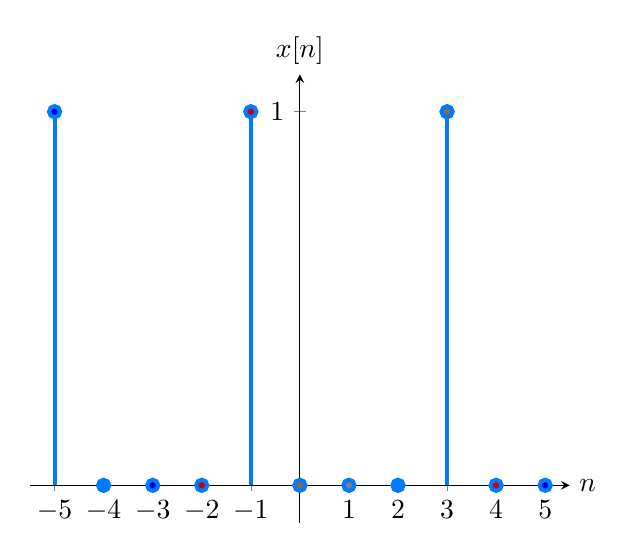
\begin{tikzpicture}
            \begin{axis}[
                xmin= -5.5, xmax= 5.5,
                ymin= -0.1, ymax = 1.1,
                xlabel={$n$}, ylabel={$x[n]$},
                axis lines = middle,
                xlabel style={at={(axis cs:5.5,0)}, anchor=west},
                ylabel style={at={(axis cs:0,1.1)}, anchor=south},
                xtick={-5,-4,...,5},
                ytick={1},
            ]
                \foreach \n in {-5,-1,3} {
    \addplot+[ycomb, mark=*, lightblue, line width=1.5] coordinates {(\n,1)};
  }
                \foreach \n in {-4,-3,-2,0,1,2,4,5} {
    \addplot+[ycomb, mark=*, lightblue, line width=1.5] coordinates {(\n,0)};
  }
            \end{axis}
        \end{tikzpicture}
       \end{center}
    Periodo: $N=4\implies \omega_0=\dfrac{2\pi}{N}=\dfrac{2\pi}{4}=\dfrac{\pi}{2}$

    $
\begin{aligned}
    a_k&=\dfrac{1}{n}\cdot \sum_{n=<N>}x[n]e^{-jk\omega_0n}=\dfrac{1}{4}\sum_{n=-1}^{2} \delta[n+1]\cdot e^{-jk\frac{\pi}{2} n} =\dfrac{1}{4}\sum_{n=-1}^{2} \delta[n+1]e^{jk\frac{\pi}{2} }=\dfrac{e^{jk\frac{\pi}{2} } }{4}\lbb{\sum_{n=-1}^{2} \delta[n+1]}{1}=\dfrac{1}{4}e^{jk\frac{\pi}{2} } \\
       &= \dfrac{1}{4}\cdot \left( e^{j\frac{\pi}{2} }  \right) ^k=\dfrac{1}{4}\cdot \left[ \tozero{\cos\left( \dfrac{\pi}{2} \right) } +j\cdot \sin\left( \dfrac{\pi}{2} \right)  \right] ^k=\dfrac{1}{4}\cdot j^k=\dfrac{j^k}{4} \\
\end{aligned}
    $

\item \lb{Calcular los coeficientes del desarrollo en series de Fourier \[
            x[n]=\sum_{m=-\infty}^{\infty} \prod\left( \dfrac{n-mN}{2N_1+1} \right) 
\] } 

$
\begin{aligned}
    a_k&=\dfrac{1}{N}\sum_{n=<N>} x[n]\cdot e^{-jk\frac{2\pi}{N} n} =\dfrac{1}{N}\sum_{n=-N_1}^{N_1} x[n]\cdot e^{-jk\frac{2\pi}{N} n} =\dfrac{1}{N}\sum_{n=-N_1}^{N_1} \left( e^{-jk\frac{2\pi}{N} }  \right) ^n=\dfrac{1}{N}\cdot \dfrac{e^{jk\frac{2\pi}{N} N_1} -e^{-jk\frac{2\pi}{N} N_2} }{1-e^{-jk\frac{2\pi}{N} } }\\
       &= \dfrac{1}{N}\cdot \dfrac{\left( e^{-jk\frac{\pi}{N} } \cdot \left( e^{jk\frac{2\pi}{N} N_1}\cdot e^{jk\frac{\pi}{N} } -e^{-jk\frac{2\pi}{N} N_1} \cdot e^{-jk\frac{2\pi}{N} } e^{jk\frac{\pi}{N} }   \right)  \right) }{e^{-jk\frac{\pi}{N}} \left( e^{jk\frac{\pi}{N} } -e^{-jk\frac{\pi}{N} }  \right) }=\dfrac{1}{N}\cdot \dfrac{e^{jk\frac{\pi}{N} (2N_1+1)} -e^{-jk\frac{\pi}{N} (2N_1+1)} }{e^{jk\frac{\pi}{N} } -e^{-jk\frac{\pi}{N} } } \\
       &= \dfrac{1}{N}\cdot \dfrac{\sin\left( k\frac{\pi}{N} (2N_1+1) \right) }{\sin\left(   k\frac{\pi}{N}\right)} \\
\end{aligned}
$
\newpage
\item \lb{Obtener el espectro de la secuencia discreta \[
            x[n]=a^nu[n],\quad|a|<1
\] } 

$X(e^{j\omega} )=\sum_{n=0}^{\infty} a^n \cdot  e^{-j\omega n}=\sum_{n=0}^{\infty} (a\cdot e^{-j\omega} )^n=\dfrac{1-(a\cdot e^{-j\omega} )^{\infty+1}}{1-a\cdot e^{-j\omega} }=\dfrac{1}{1-a\cdot e^{-j\omega} }$
\item \lb{Obtener el espectro de la secuencia discreta \[
            x[n]=\prod\left( \dfrac{n}{2N_1+1} \right) 
\] } 
$X(e^{j\omega} )=\sum_{n=-N_1}^{N_1} e^{-j\omega n}= \dfrac{e^{j\omega N_1} -e^{-j\omega(N_1+1)} }{1-e^{-j\omega} }$
\item \lb{Obtener el espectro de la secuencia discreta \[
x[n]=\cos\left( \dfrac{2\pi}{5}n \right) 
\] } 

$x[n]=\cos\left( \dfrac{2\pi}{5}n \right)\implies \dfrac{e^{\frac{2\pi}{5} jn} +e^{-\frac{2\pi}{5} jn} }{2}\implies \begin{cases}
    a_1=\tfrac{1}{2} \\
    a_{-1}=\tfrac{1}{2} 
\end{cases}$ 

$X(e^{j\omega} )=\sum_k 2\pi a_k\cdot \delta(\omega-k\omega_0)=2\pi\cdot \dfrac{1}{2}^\delta\left( \omega-\dfrac{2\pi}{5} \right) +2\pi\cdot \dfrac{1}{2}\cdot \delta\left( \omega+\dfrac{2\pi}{5} \right) =\pi\cdot \left( \delta\left( \omega-\dfrac{2\pi}{5} \right) +\delta\left( \omega+\dfrac{2\pi}{5} \right)  \right) $
\item \lb{Obtener el espectro de la secuencia discreta \[
            x[n]=\sum_{m=-\infty}^{\infty} \delta[n-mN]
\] } 
$X(e^{j\omega} )=\sum_k 2\pi \cdot a_k\cdot \delta(\omega-k\omega_0)=\sum_k 2\pi\cdot \dfrac{1}{N}\cdot \delta\left( \omega-k \dfrac{2\pi}{N} \right)$
\item \lb{Obtener el espectro aplicando propiedades \[
            x[n]=u[n]
\] } 

$\begin{array}{l}
    X(e^{j\omega} )=\sum_{n=0}^{\infty} e^{-j\omega n}=\dfrac{1-e^{-j\omega(\infty+1)} }{1-e^{-j\omega} }=\dfrac{1}{1-e^{-j\omega} } \\
    \begin{array}{ll}
        z[n]=\delta[n]\to Z(e^{j\omega} )=1 & X(e^{j\omega} )=\dfrac{Z(e^{j\omega} )}{1-e^{-j\omega} }+\pi\cdot Z(e^{j\cdot 0} )\cdot \sum_{k=-\infty}^{\infty} \delta(\omega-2\pi k)\\
        x[n]=\sum_{m=-\infty}^{\infty} z[m]=u[n] & X(e^{j\omega} )=\dfrac{1}{1+e^{-j\omega} }+\pi\cdot \sum_{k=-\infty}^{\infty} \delta(\omega-2\pi k)
    \end{array}
\end{array}$
\newpage
\item \lb{Obtener el espectro aplicando propiedades \[
            x[n]=\left( \dfrac{1}{2} \right) ^{|n-1|}
\] } 
\begin{minipage}{0.45\textwidth}
    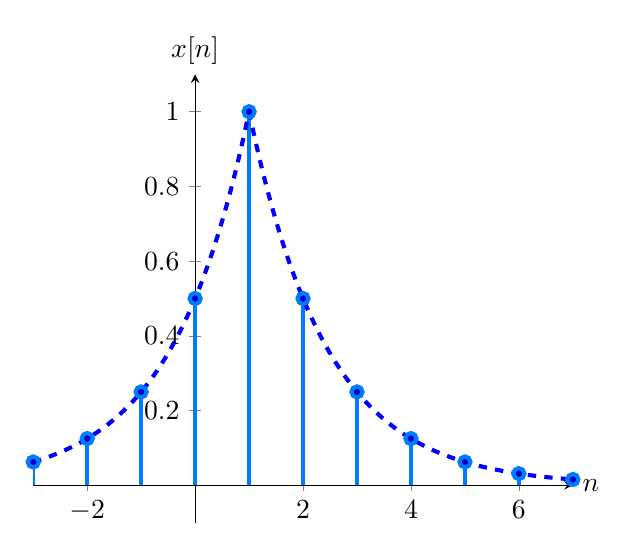
\begin{tikzpicture}
        \begin{axis}[
            xmin= -3, xmax= 7,
            ymin= -0.1, ymax = 1.1,
            xlabel={$n$}, ylabel={$x[n]$},
            axis lines = middle,
            xlabel style={at={(axis cs:7,0)}, anchor=west},
            ylabel style={at={(axis cs:0,1.1)}, anchor=south},
        ]
            \pgfmathsetmacro{\mysamples}{7-(-3)+1}
            \addplot+[ycomb, mark=*, lightblue, line width=1.5, domain=-3:7, samples=\mysamples] {(0.5)^(abs(x-1))};
            \addplot[blue, dashed, line width=1.5, domain=-3:7, samples=1000] {(0.5)^(abs(x-1))};
        \end{axis}
    \end{tikzpicture}
\end{minipage}\qquad
\begin{minipage}{0.45\textwidth}
    $\begin{aligned}
        X(e^{j\omega} )&= \left( \dfrac{1}{2} \right) \cdot \left( \left( \dfrac{1}{2} \right)^{-n}\cdot u[-n]  \right) + \left( \left( \dfrac{1}{2} \right) ^{n-1}\cdot u[n-1] \right)  \\
        &= \dfrac{1}{2}\cdot \dfrac{1}{1-\frac{1}{2} \cdot e^{j\omega} }+\dfrac{1}{1-\frac{1}{2} e^{-j\omega} }\cdot e^{-j\omega}  \\
    \end{aligned}$
\end{minipage}

\item \lb{Obtener el espectro aplicando propiedades \[
            x[n]=2^n\sin\left( \dfrac{\pi}{4}n \right)u[-n]
\] } 
$x[n]=\dfrac{1}{2j}\cdot \left( 2^n\cdot u[-n]\cdot e^{j\frac{\pi}{4} n}  \right) -\left( 2^n \cdot u[-n]\cdot e^{-j\frac{\pi}{4} n}  \right) $ 

$x_1[n]=2^n\cdot u[-n]\implies X_1(e^{j\omega} )=\dfrac{1}{1-2e^{j\omega} }$ 

$X(e^{j\omega} )=\dfrac{1}{2j}\cdot \left( X_1\left(e^{j\left(\omega-\frac{\pi}{4} \right)} \right) -X_1\left(e^{j\left( \omega+\frac{\pi}{4}  \right) } \right)\right) =\dfrac{1}{2j}\cdot \left( \dfrac{1}{1-\frac{1}{2}\cdot e^{j\left( \omega-\frac{\pi}{4} \right)} }-\dfrac{1}{1-\frac{1}{2} e^{j\left( \omega+\frac{\pi}{4}  \right) } } \right) $
\item \lb{Obtener el espectro aplicando propiedades \[
            x[n]=n\left( \dfrac{1}{3} \right) ^{|n|}
\] }
\begin{minipage}{0.45\textwidth}
    \begin{tikzpicture}
        \begin{axis}[
            xmin= -5, xmax= 5,
            ymin= -0.7, ymax = 0.7,
            xlabel={$n$}, ylabel={$x[n]$},
            axis lines = middle,
            xlabel style={at={(axis cs:5,0)}, anchor=west},
            ylabel style={at={(axis cs:0,0.7)}, anchor=south},
            ytick={-0.5,0.5}
        ]
            \pgfmathsetmacro{\mysamples}{5-(-5)+1}
            \addplot+[ycomb, mark=*, lightblue, line width=1.5, domain=-5:5, samples=\mysamples] {x*(1/3)^(abs(x))};
        \end{axis}
    \end{tikzpicture}
\end{minipage}\quad
\begin{minipage}{0.45\textwidth}
$
\begin{aligned}
    x[n]&=\begin{cases}
    n\left( \frac{1}{3}  \right) ^n, & n\ge 0\\
    n\left( \frac{1}{3}  \right) ^{-n} & n<0
\end{cases}\\
&=  \begin{cases}
    n\left( \frac{1}{3}  \right)^n, & n\ge 0\\
    n\cdot 3^n, & n<0
\end{cases}\\
\end{aligned}
$
\[
    x[n]=x_1[n]+x_2[n]
\]
\end{minipage}

donde:
\begin{itemize}[label=\textbullet]
    \item $x_1[n]=n\left( \dfrac{1}{3} \right) ^n u[n]\implies X_1(e^{j\omega} )=\dfrac{\frac{1}{3} e^{j\omega} }{\left(1-\frac{1}{3} e^{j\omega} \right)^2}$
    \item $x_2[n]=n\cdot 3^nu[-n-1]=-n\cdot 3^nu[n+1]=-x_1[-n]\implies X_2(e^{j\omega} )=-X_1(e^{-j\omega} )=-\dfrac{\frac{1}{3} e^{-j\omega} }{\left( 1-\frac{1}{3} e^{-j\omega}  \right) ^2}$
\end{itemize}
\[
X(e^{j\omega} )=X_1(e^{j\omega} )+X_2(e^{j\omega} )=\dfrac{\frac{1}{3} e^{j\omega} }{\left( 1-\frac{1}{3} e^{j\omega}  \right) ^2}-\dfrac{\frac{1}{3}e^{-j\omega}}{\left( 1-\frac{1}{3} e^{-j\omega} \right) ^2}
\] 
\newpage
\item \lb{Ejemplo de sistema LTI discreto causal descrito mediante una ecuación en diferencias lineal con coeficientes constantes: \[
            y[n]-\dfrac{3}{4}y[n-1]+\dfrac{1}{8}y[n-2]=2x[n]
\] } 
$y[n]-\dfrac{3}{4}y[n-1]+\dfrac{1}{8}y[n-2]=2x[n]\implies Y(e^{j\omega} )-\dfrac{3}{4}Y(e^{j\omega} )\cdot e^{-j\omega} +\dfrac{1}{8}Y(e^{j\omega} )\cdot e^{-2j\omega}=2\cdot X(e^{j\omega} ) $
    
$H(e^{j\omega} )=\dfrac{Y(e^{j\omega} )}{X(e^{j\omega} )}=\dfrac{2}{1-\frac{3}{4} e^{-j\omega} +\frac{1}{8} e^{-2j\omega} }=\{e^{j\omega}=z \}=\dfrac{2}{1-\frac{3}{4} z^{-1}+\frac{1}{8}z^{-2}} $

$z^2\cdot \left( 1-\dfrac{3}{4} z^{-1}+\dfrac{1}{8}z^{-2} \right) =z^2-\dfrac{3}{4}z+\dfrac{1}{8}=0\implies z=\dfrac{\frac{3}{4} \pm\sqrt{\left( -\frac{3}{4}  \right) ^2-4\cdot 1\cdot \frac{1}{8} } }{2\cdot 1}=\dfrac{\frac{3}{4} \pm\sqrt{\frac{1}{16}} }{2}=\begin{cases}
    \dfrac{\frac{3}{4} +\frac{1}{4} }{2}=\dfrac{1}{2}\\
    \dfrac{\frac{3}{4} -\frac{1}{4} }{2}=\dfrac{1}{4}\\
\end{cases}$

$H(e^{j\omega} )=\dfrac{A}{1-\frac{1}{2} z^{-1}}+\dfrac{B}{1-\frac{1}{4} z^{-1}}=\dfrac{4}{1-\frac{1}{2}e^{-j\omega}  }-\dfrac{2}{1-\frac{1}{4} e^{-j\omega} }$

$\begin{array}{l}
    A=H(z)\cdot \left( 1-\dfrac{1}{2}z^{-1} \right)\Bigg|_{z=\frac{1}{2}}=\dfrac{2}{1-\frac{1}{4} z^{-1}}\Bigg|_{z=\frac{1}{2} }=4\\
    B=H(z)\cdot \left( 1-\dfrac{1}{4}z^{-1} \right)\Bigg|_{z=\frac{1}{4}}=\dfrac{2}{1-\frac{1}{2} z^{-1}}\Bigg|_{z=\frac{1}{4} }=-2\\
\end{array}$

$h[n]=4\cdot \left( \dfrac{1}{2} \right) ^{n}u[n]-2\cdot \left( \dfrac{1}{4} \right) ^{n}u[n]=2\cdot \left( \dfrac{1}{2} \right) ^{n}\left( 2-\left( \dfrac{1}{2} \right) ^{n} \right) u[n]$
\item \lb{Calcular la DFT de $x[n]=\cos\left( \dfrac{\pi}{2}n \right) ,\:0\le n\le 3$} 

$a_k=\dfrac{1}{N}\cdot \sum_{n=0}^{N-1} \cos\left( \dfrac{\pi}{2}n \right) e^{-j\omega kn}=\dfrac{1}{4}\sum_{n=0}^{3} \cos\left( \dfrac{\pi}{2}n \right) e^{-j\frac{2\pi}{4} kn}=\dfrac{1}{4}\sum_{n=0}^{3} \cos\left( \dfrac{\pi}{2}n \right) e^{-j\frac{\pi}{2} kn}$ 

$
\begin{aligned}
X(e^{j\omega} )&=\sum_{n=0}^{3} \cos\left( \dfrac{\pi}{2}n \right) e^{-j\omega kn}=\sum_{n=0}^{3} \cos\left( \dfrac{\pi}{2}n \right) e^{-j\frac{2\pi}{4} kn} =\sum_{n=0}^{3} \cos\left( \dfrac{\pi}{2}n \right) e^{-j\frac{\pi}{2} kn} =1+0+(-1)\cdot (-1)^k +0\\
               &\implies \begin{cases}
    0, & \text{si }k=0,2\\
    2, & \text{si }k=1,3
\end{cases}
\end{aligned}
$
\item \lb{Calcular la DFT de $x[n]=2^n,\: 0\le n\le 3$} 

    $X[k]=\sum_{n=0}^{3} 2^ne^{-j\frac{2\pi}{4} kn}=\sum_{n=0}^{3} 2^ne^{-j\frac{\pi}{2} kn} =\sum_{n=0}^{3} \left( 2\cdot \left( e^{-j\frac{\pi}{2} }  \right) ^k \right) ^n=\sum_{n=0}^{3} (2\cdot (-j)^k)^n =\begin{cases}
        k=0:1+2+4+8=15\\
        k=1:1-2j-4+8j=-3+6j\\
        k=2:1-2+4-8=-5\\
        k=3:1+2j-4-8j=-3-6j
    \end{cases}$
\item \lb{Calcular la DFT de $x[n]=\prod\left( \dfrac{n-2}{5} \right) $} 

    $x[k]=\sum_{n=0}^{4} e^{-j\frac{2\pi}{5} kn} =\sum_{n=0}^{4} \left( \left( e^{-j\frac{2\pi}{5} }  \right) ^k \right) ^n=\begin{cases}
        k=0:5\\
        k=1:\left( e^{-\frac{2\pi}{5} }  \right) ^n\to e^{-j\frac{2\pi}{5} } =0\\
        k=2:0\\
        k=3:0\\
        k=4:0
    \end{cases}$
    \newpage
\item \lb{Calcular $z[n]=x[n]\circledast x[n]$, siendo $x[n]=\prod\left( \dfrac{n-1}{3} \right) $} 

    $Z[k]=X[k]\cdot X[k]=3\cdot \delta[k]\cdot 3\cdot \delta[k]=9\delta[k]$

    $z[n]=\dfrac{1}{3}\sum_{k=0}^{2} 9\delta[k]=\dfrac{9}{3}\cdot 1=3$ 

    $z[n]=3\prod\left( \dfrac{n-1}{3} \right) $ 
    \begin{center}
        \begin{tikzpicture}
            \begin{axis}[
                xmin= -5, xmax= 5,
                ymin= -1, ymax = 4,
                xlabel={$n$}, ylabel={$x[n]$},
                axis lines = middle,
                xlabel style={at={(axis cs:5,0)}, anchor=west},
                ylabel style={at={(axis cs:0,4)}, anchor=south},
            ]
                \pgfmathsetmacro{\mysamples}{5-(-5)+1}
                \addplot+[ycomb, mark=*, lightblue, line width=1.5, domain=-5:5, samples=\mysamples] {3*rect((x-1)/3)};
            \end{axis}
        \end{tikzpicture}
    \end{center}
\end{enumerate}
\end{document}
